\chapter{Конструкторский раздел}
\label{cha:design}

\section{IDEF0}

На рисунке \ref{fig:idef0} приведена диаграмма состояний IDEF0 нулевого уровня, а на рисунке \ref{fig:idef1} --- диаграмма состояний IDEF0 первого уровня.

\begin{figure}[ph!]
	\center{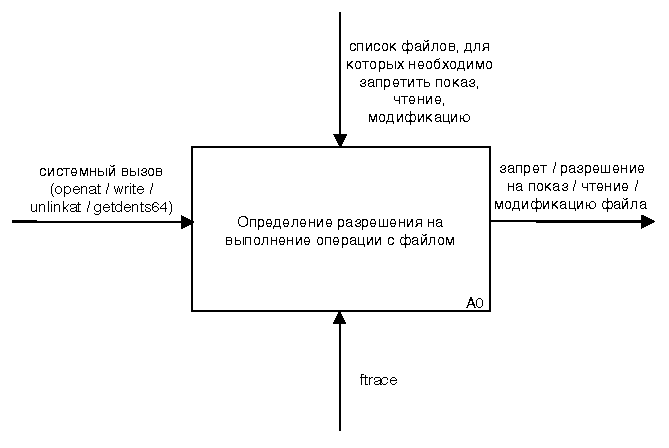
\includegraphics[scale=1.3]{img/idef0_0.pdf}}
	\caption{Диаграмма состояний IDEF0 нулевого уровня}
	\label{fig:idef0}
\end{figure}

\begin{figure}[ph!]
	\center{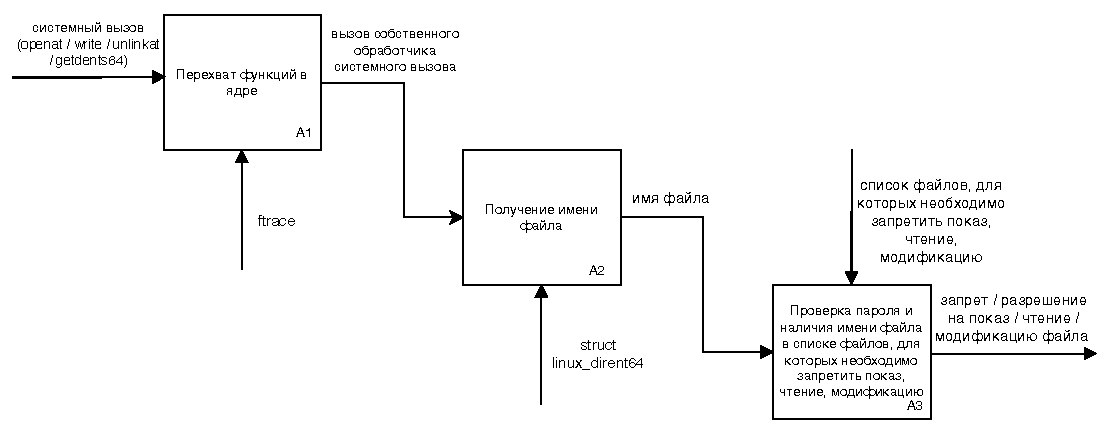
\includegraphics[scale=0.9]{img/idef0_1.pdf}}
	\caption{Диаграмма состояний IDEF0 первого уровня}
	\label{fig:idef1}
\end{figure}

\clearpage

%\section{Алгоритм создания символьного устройства}

%На рисунке \ref{fig:dev} приведена схема создания символьного устройства для ввода пароля.

%\begin{figure}[ph!]
%	\center{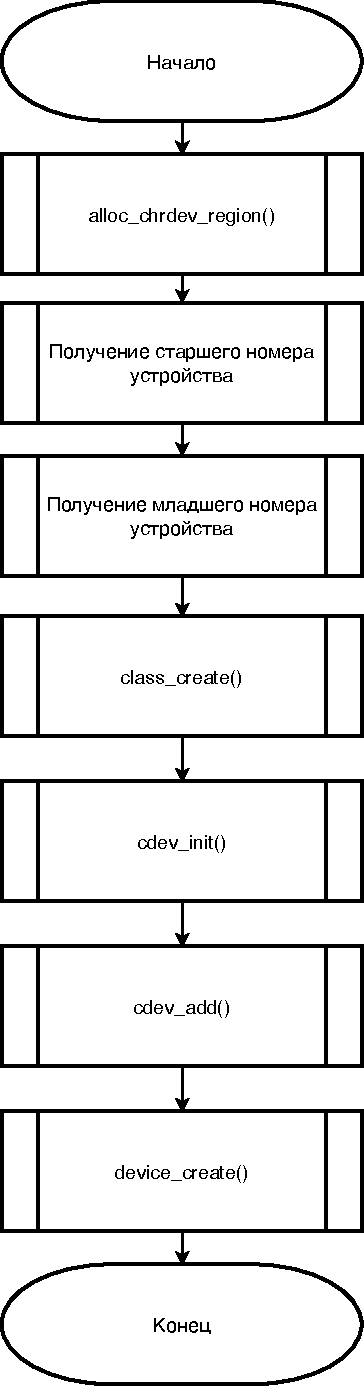
\includegraphics[scale=0.65]{img/cdev.pdf}}
%	\caption{Алгоритм создания символьного устройства}
%	\label{fig:dev}
%\end{figure}

%\clearpage

%\section{Алгоритм проверки наличия разрешения на выполнение действия с файлом}

%На рисунке \ref{fig:init} приведена схема алгоритма проверки наличия разрешения на выполнение действия с файлом.

%\begin{figure}[ph!]
%	\center{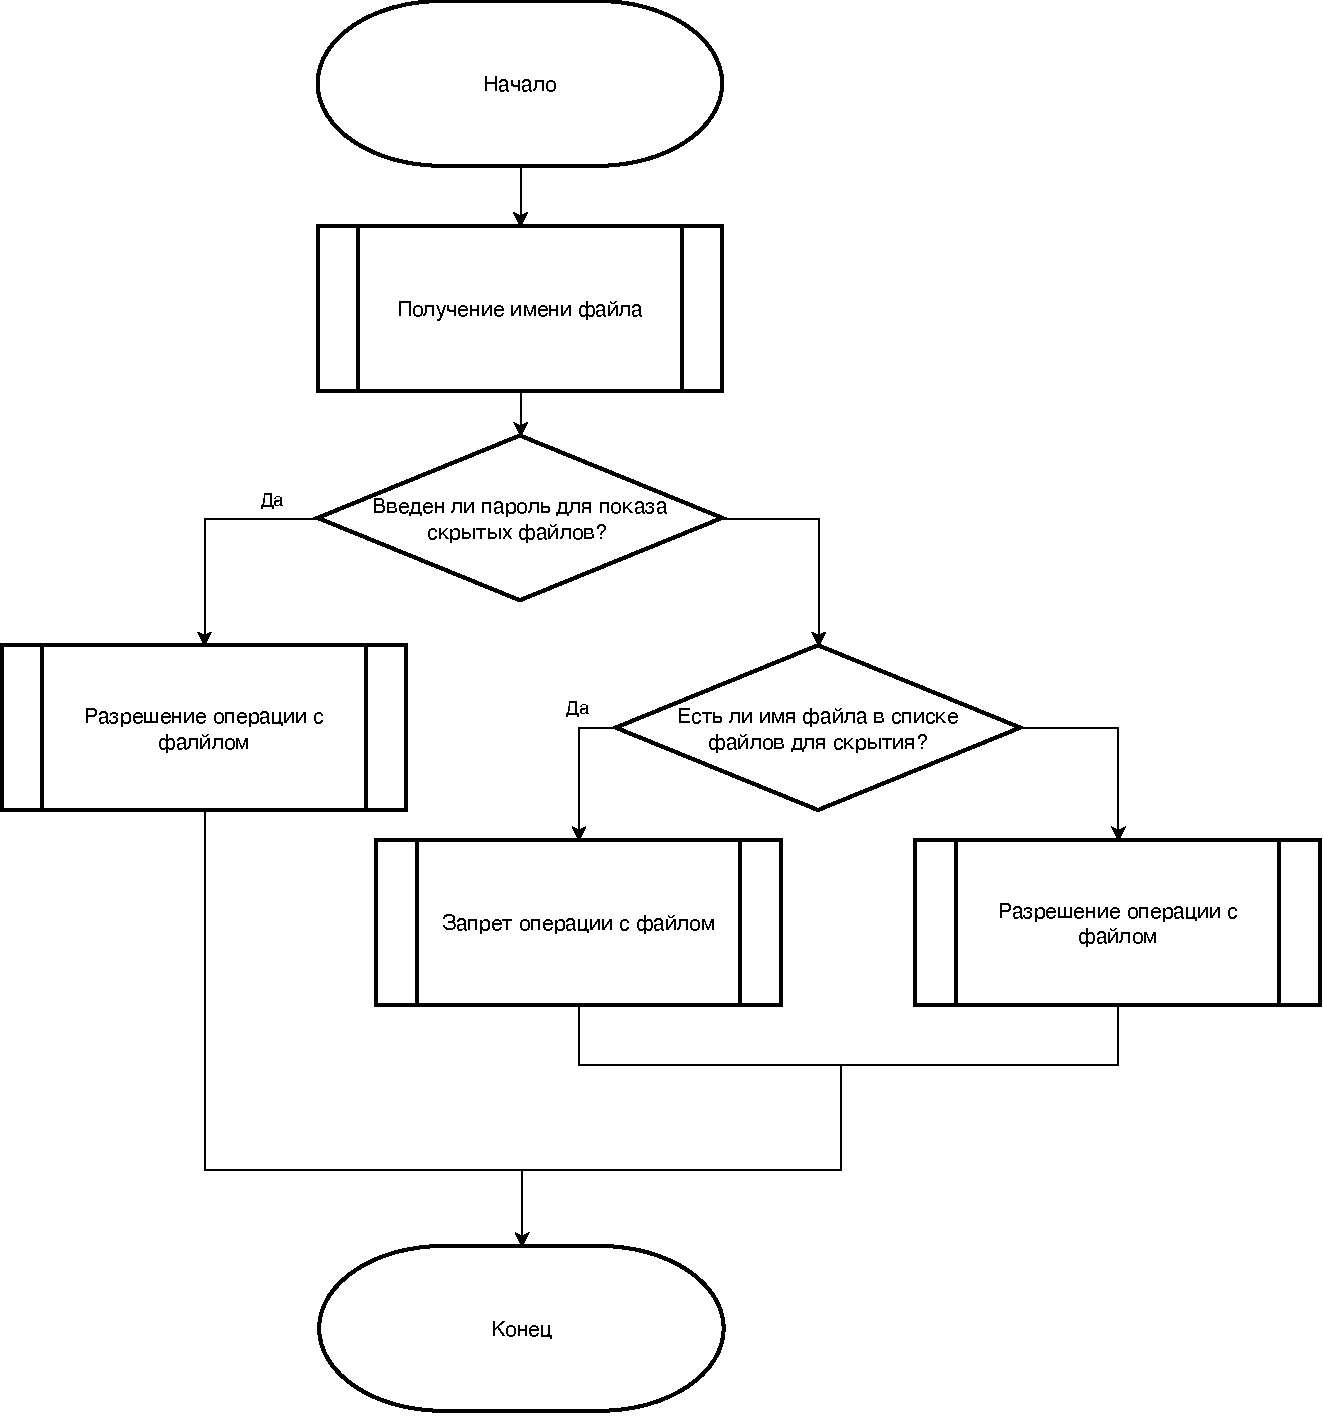
\includegraphics[scale=0.6]{img/check.pdf}}
%	\caption{Алгоритм проверки наличия разрешения на выполнение действия с файлом}
%	\label{fig:init}
%\end{figure}

%\clearpage

\section{Алгоритм проверки необходимости сокрытия файла}

На рисунке \ref{fig:getdents64} приведена схема алгоритма проверки необходимости сокрытия файла.

\begin{figure}[ph!]
	\center{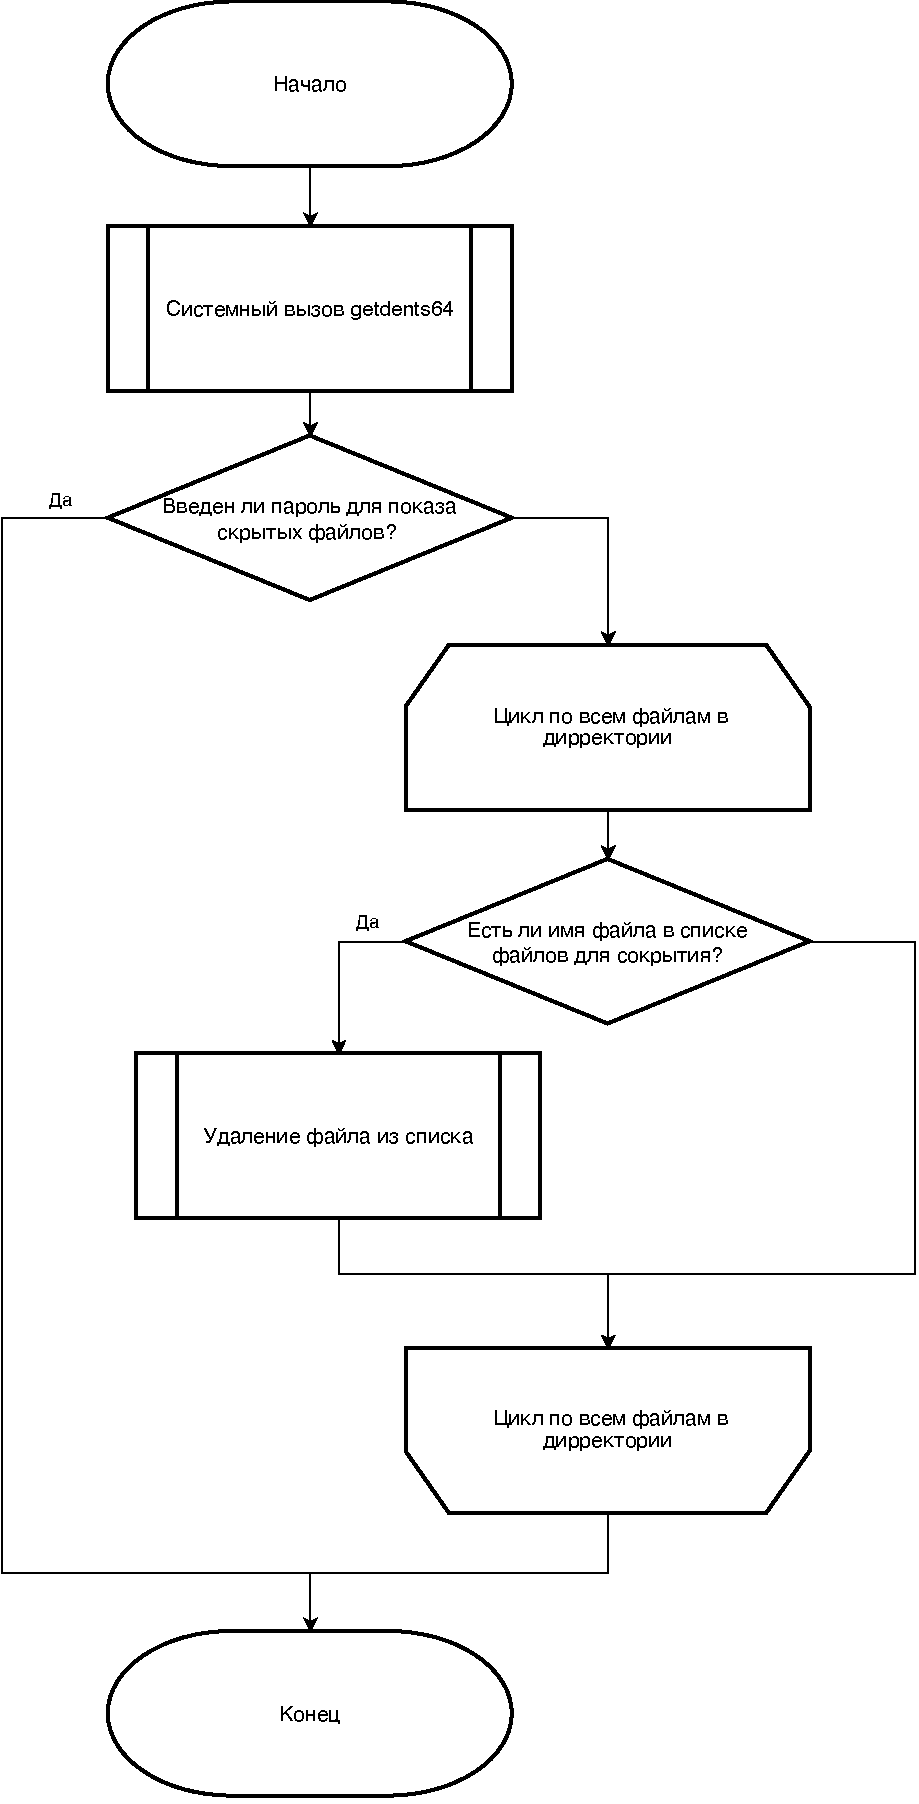
\includegraphics[scale=0.65]{img/getdents.pdf}}
	\caption{Алгоритм проверки необходимости сокрытия файла}
	\label{fig:getdents64}
\end{figure}

\clearpage

\section{Алгоритм проверки разрешения на удаление файла}

На рисунке \ref{fig:unlink} приведена схема алгоритма проверки разрешения на удаление файла.

\begin{figure}[ph!]
	\center{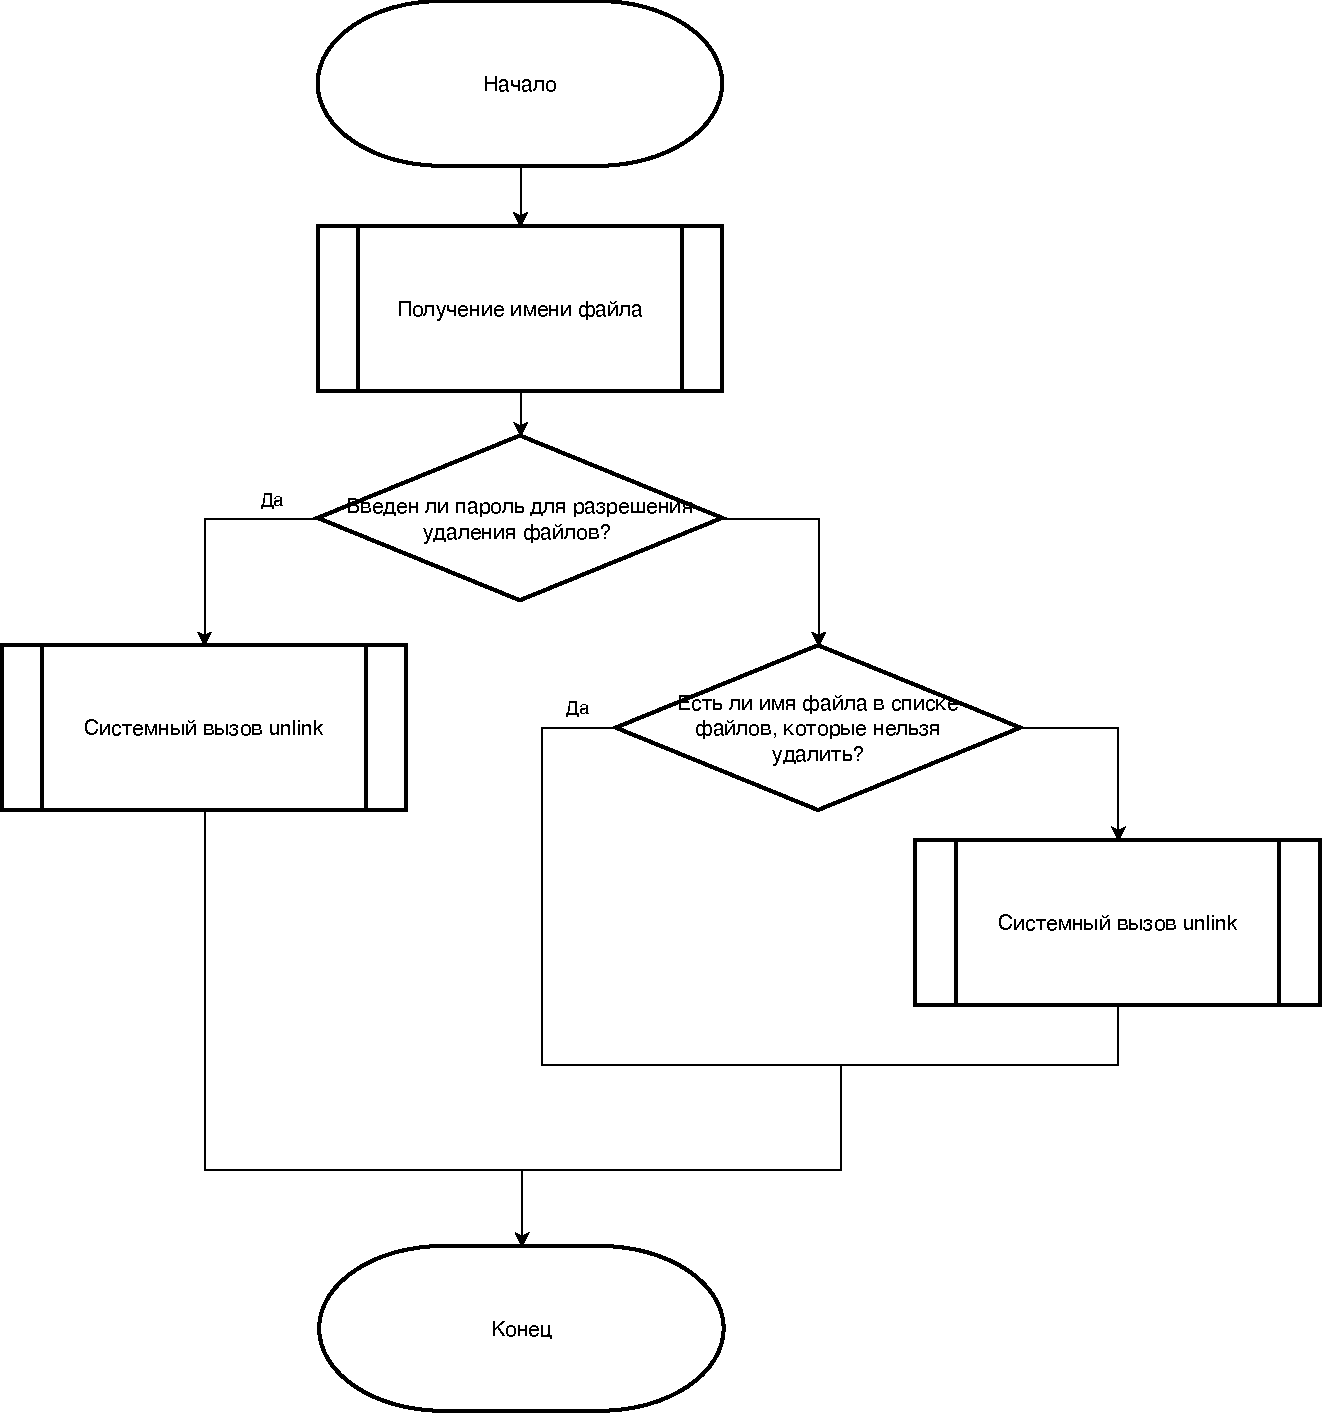
\includegraphics[scale=0.65]{img/unlink.pdf}}
	\caption{Алгоритм проверки разрешения на удаления файла}
	\label{fig:unlink}
\end{figure}

\clearpage

\section{Алгоритм проверки разрешения на запись в файл}

На рисунке \ref{fig:write} приведена схема алгоритма проверки разрешения на запись в файл.

\begin{figure}[ph!]
	\center{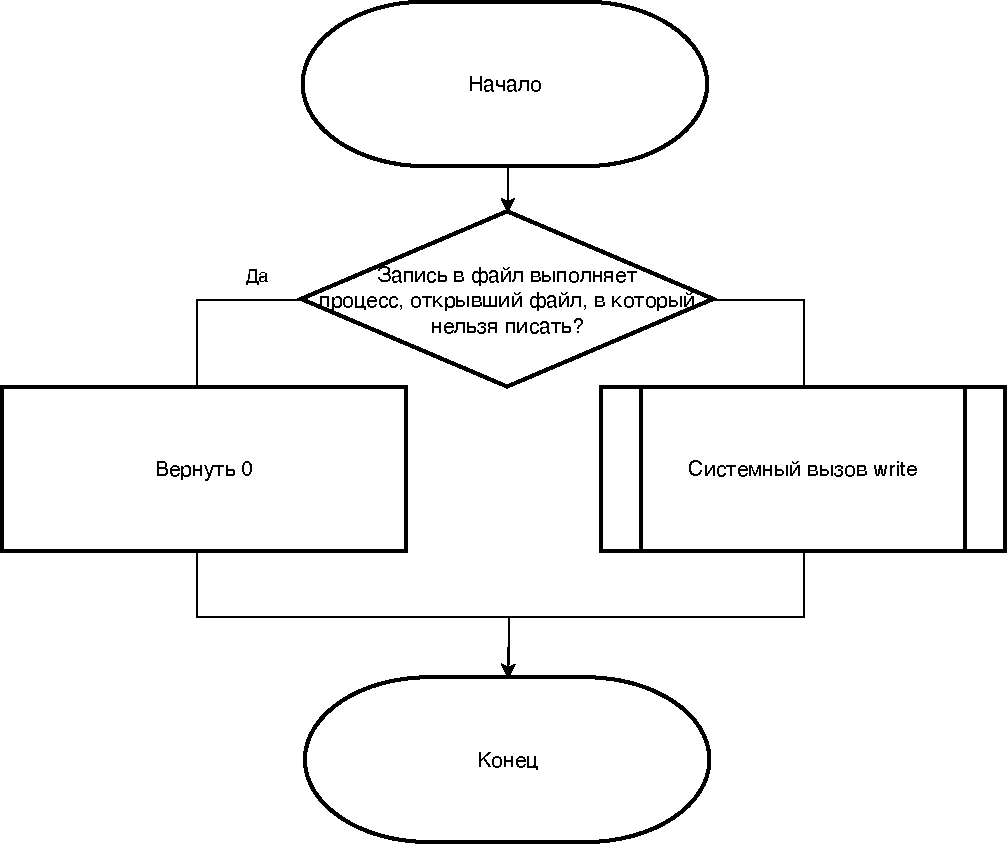
\includegraphics[scale=0.52]{img/write.pdf}}
	\caption{Алгоритм проверки разрешения на запись в файл}
	\label{fig:write}
\end{figure}

\section{Алгоритм проверки разрешения на чтение из файла}

На рисунке \ref{fig:read} приведена схема алгоритма проверки разрешения на чтение из файла.

\begin{figure}[ph!]
	\center{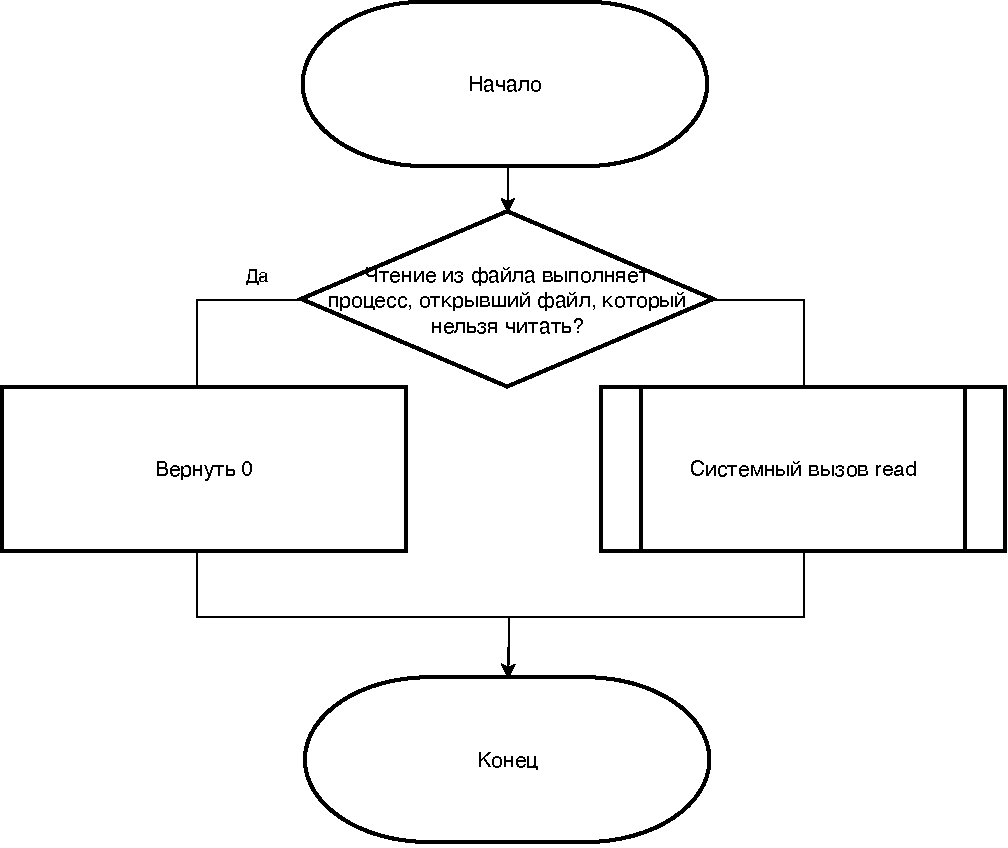
\includegraphics[scale=0.52]{img/read.pdf}}
	\caption{Алгоритм проверки разрешения на чтение из файла}
	\label{fig:read}
\end{figure}

\clearpage

\section{Структура программного обеспечения}

На рисунке \ref{fig:struct} представлена структура программного обеспечения.

\begin{figure}[ph!]
	\center{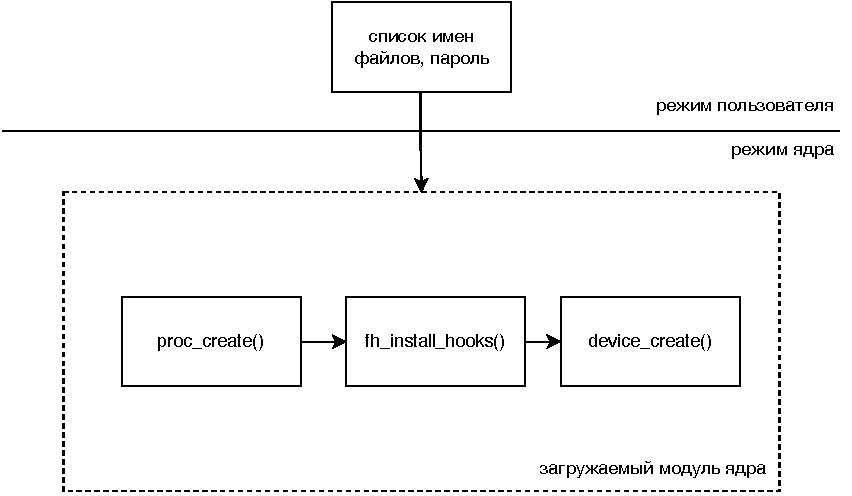
\includegraphics[scale=1]{img/structure.pdf}}
	\caption{Структура программного обеспечения}
	\label{fig:struct}
\end{figure}



